% Cramér windows at x=e^{10}, so log x=10. Lengths (log x)^lambda and means sum 1/log n were computed directly.
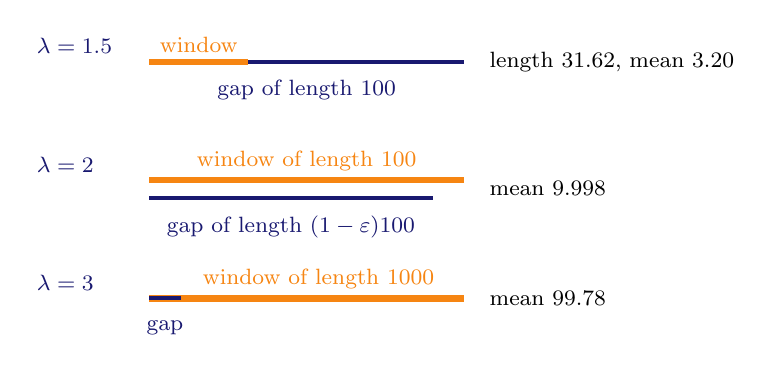
\begin{tikzpicture}[every node/.style={font=\footnotesize}]
  % lambda = 1.5. Scale: 100 -> 4cm. The window sits inside a gap of length 100.
  \node[anchor=west,MidnightBlue] at (0,3.35) {$\lambda=1.5$};
  \draw[MidnightBlue,line width=1.4pt] (1.55,3.15)--(5.55,3.15);
  \draw[BurntOrange,line width=2.4pt] (1.55,3.15)--(2.81,3.15);
  \node[below,MidnightBlue] at (3.55,3.05) {gap of length $100$};
  \node[above,BurntOrange] at (2.18,3.15) {window};
  \node[anchor=west] at (5.75,3.15) {length $31.62$, mean $3.20$};

  % lambda = 2. Same scale. Gap a little shorter than the window.
  \node[anchor=west,MidnightBlue] at (0,1.85) {$\lambda=2$};
  \draw[BurntOrange,line width=2.4pt] (1.55,1.65)--(5.55,1.65);
  \draw[MidnightBlue,line width=1.4pt] (1.55,1.42)--(5.15,1.42);
  \node[above,BurntOrange] at (3.55,1.65) {window of length $100$};
  \node[below,MidnightBlue] at (3.35,1.32) {gap of length $(1-\varepsilon)100$};
  \node[anchor=west] at (5.75,1.55) {mean $9.998$};

  % lambda = 3. Scale: 1000 -> 4cm, so a gap of 100 is 0.4cm.
  \node[anchor=west,MidnightBlue] at (0,0.35) {$\lambda=3$};
  \draw[BurntOrange,line width=2.4pt] (1.55,0.15)--(5.55,0.15);
  \draw[MidnightBlue,line width=1.6pt] (1.55,0.15)--(1.95,0.15);
  \node[above,BurntOrange] at (3.7,0.15) {window of length $1000$};
  \node[below,MidnightBlue] at (1.75,-0.02) {gap};
  \node[anchor=west] at (5.75,0.15) {mean $99.78$};
\end{tikzpicture}
